\chapterimage{blue23.jpeg} % Imagen de encabezado de capítulo
\chapterspaceabove{6.75cm} % Espacio en blanco desde la parte superior de la página hasta el título del capítulo en las páginas del capítulo
\chapterspacebelow{6.25cm} % Cantidad de espacio en blanco vertical desde el margen superior hasta el comienzo del texto en las páginas de los capítulos

%------------------------------------------------

\chapter{ÁLGEBRA BOOLEANA}\label{chap:4}

\tcbsidebyside[title=George Boole,
      sidebyside adapt=left,
      bicolor,
      colback=white,
      colbacklower=jblueinner,
      colframe=jblueleft,
      fonttitle=\bfseries,
      center title,
      fuzzy shadow = {0pt}{-3pt}{-0.5pt}{0.5pt}{black!35},
]{%
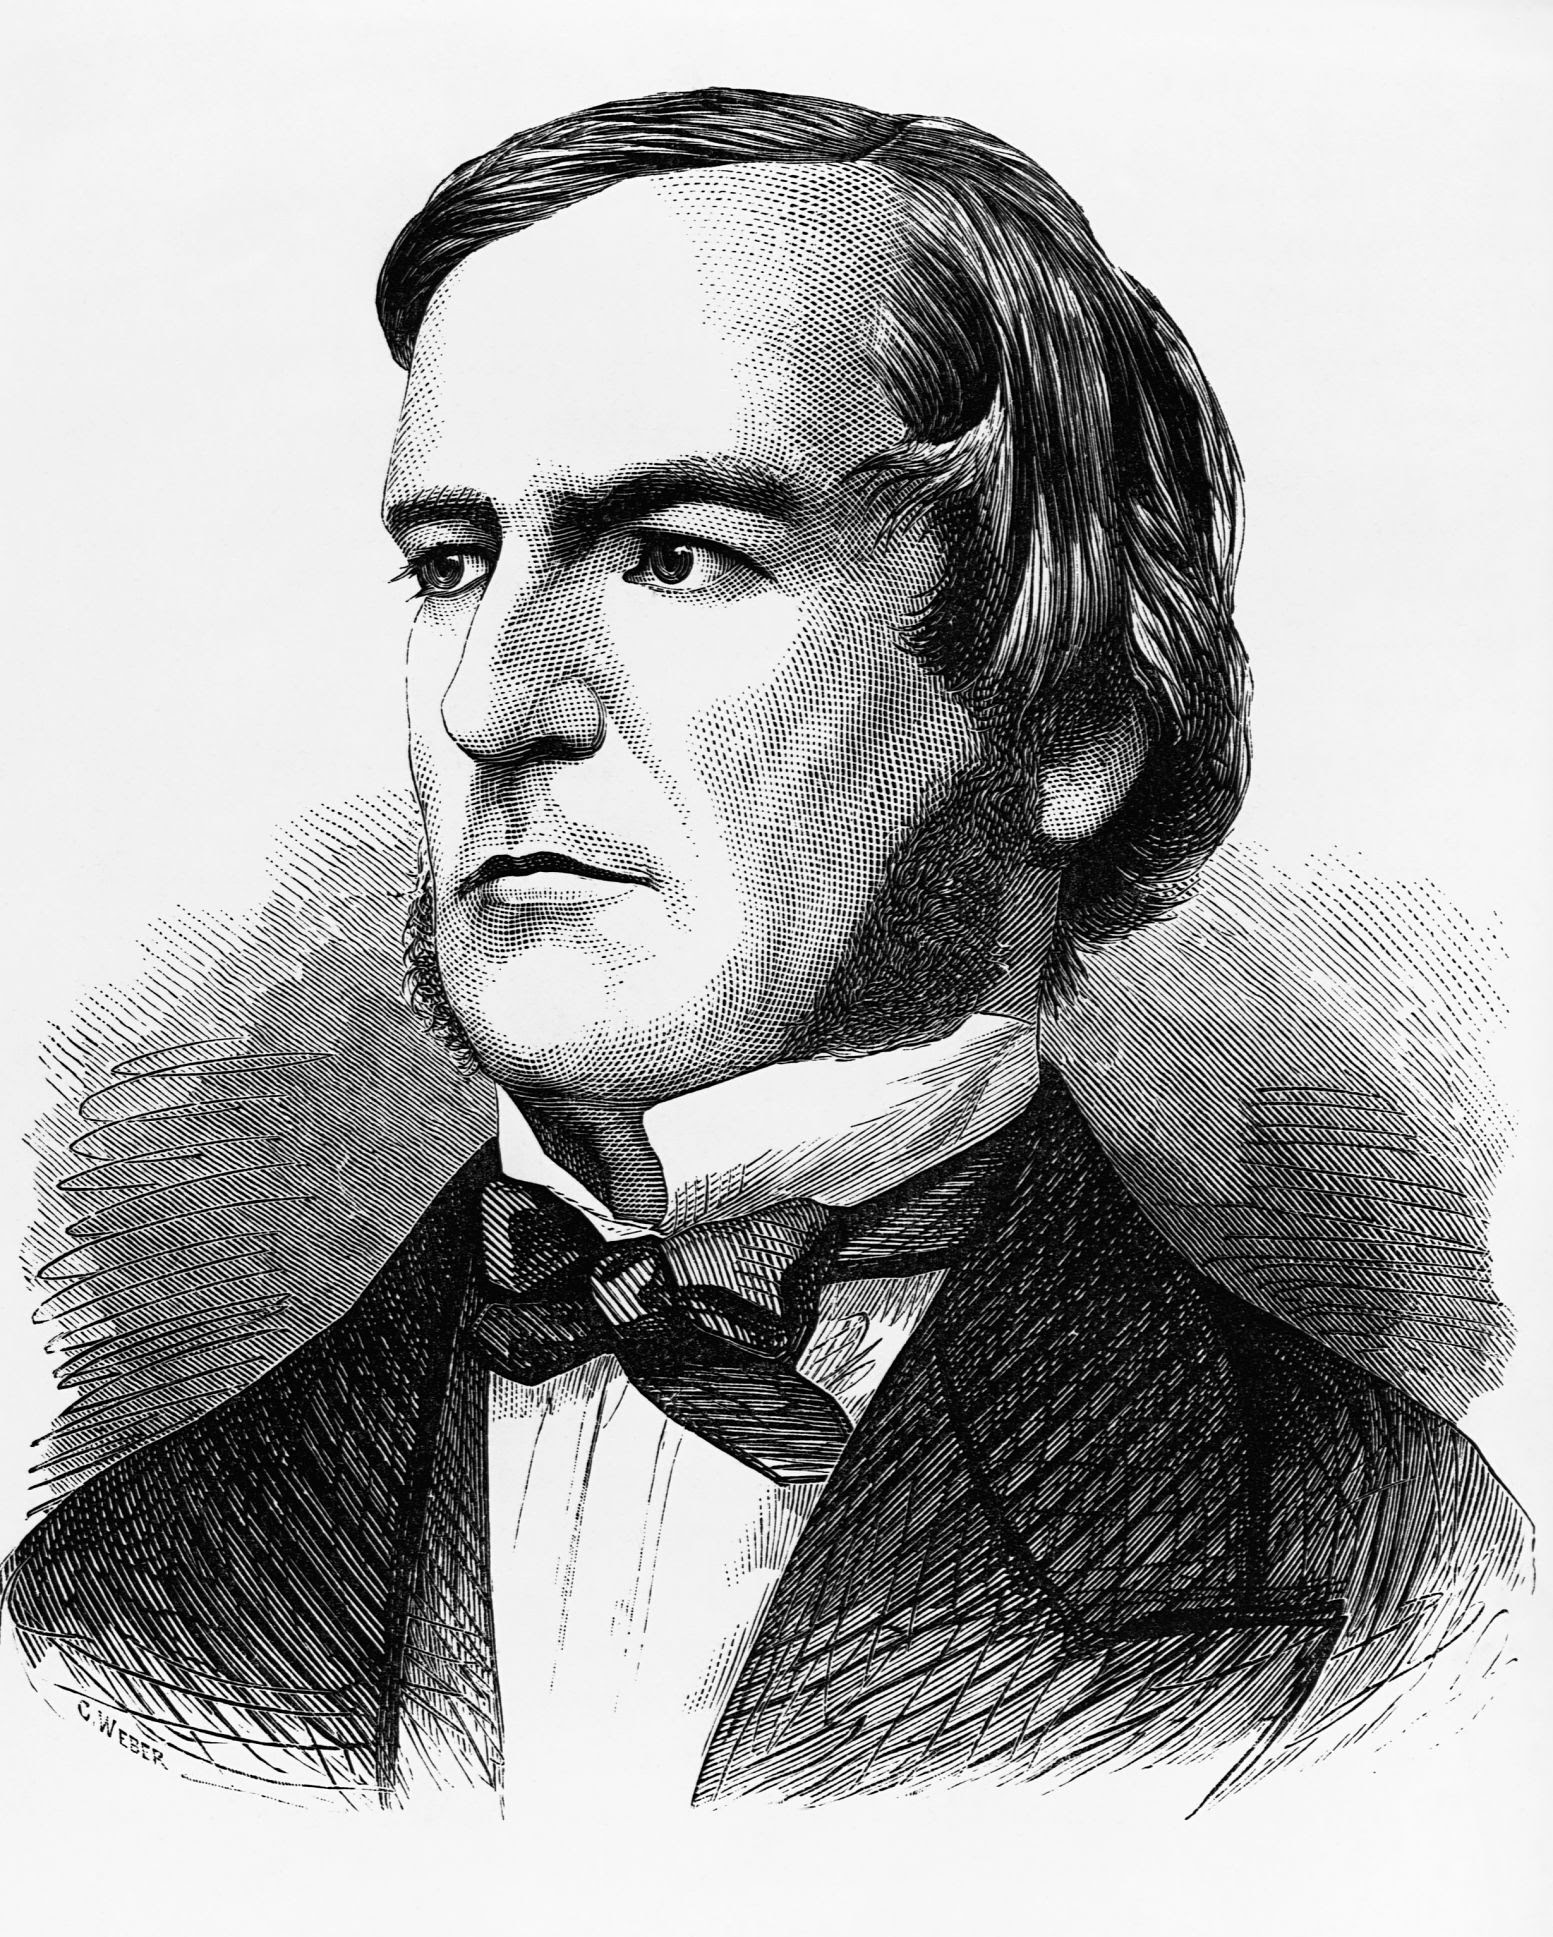
\includegraphics[width=0.36\textwidth]{Images/IMG_0373.jpeg}
}{%
George Boole fue un matemático británico nacido el 2 de noviembre de 1815 en Lincoln, Inglaterra, y fallecido el 8 de diciembre de 1864 en Ballintemple, Irlanda. Es conocido por sus contribuciones pioneras en el campo de la lógica y el álgebra. En 1847, publicó su obra “The Mathematical Analysis of Logic”, donde presentó un sistema algebraico que permitía representar el razonamiento lógico mediante símbolos y ecuaciones, un precursor del Álgebra Booleana, fundamental en la informática y la electrónica. Sus leyes lógicas, conocidas como las “Leyes de Boole”, siguen siendo fundamentales en la teoría de circuitos digitales y la programación. George Boole dejó un legado duradero en las matemáticas y la informática, y su trabajo continúa siendo relevante en la era digital.
}

El Álgebra Booleana, nombrada en honor a George Boole, es un campo fundamental en las Matemáticas Discretas que encuentra sus raíces en la lógica y la teoría de conjuntos. Esta rama de las matemáticas se ha convertido en un pilar esencial en la informática y la ingeniería eléctrica, ya que proporciona un marco formal para el análisis y la manipulación de sistemas que pueden tener solo dos estados: verdadero o falso, 1 o 0 respectivamente. Además, una característica distintiva, es su capacidad para representar problemas complejos mediante ecuaciones booleanas y simplificar estas ecuaciones utilizando reglas algebraicas específicas. Esto es esencial para diseñar circuitos digitales, construir algoritmos eficientes y resolver problemas lógicos de manera sistemática.\\


El Álgebra Booleana se basa en un conjunto de operaciones fundamentales, las cuales son AND, OR y NOT, que permiten combinar y transformar variables booleanas. A partir de estas operaciones básicas, se pueden derivar muchas otras, como XOR (o exclusivo), NAND (NO Y), NOR (NO O), entre otras.

\newpage

\section{Funciones booleanas: Formas normales disyuntiva y conjuntiva}

Como tema preliminar, debemos saber que un interruptor eléctrico puede encenderse (permitiendo el flujo de corriente) o apagarse (evitando el flujo de corriente). Es decir

\begin{center}
    \begin{tabular}{ccccl}
        \begin{circuitikz}
            \draw (1,0) to[short,-*] (2,0);
            \draw[very thick] (2,0) -- +(40:0.8);
            \draw (2.75,0) to[short,*-] (4,0);
        \end{circuitikz} & & 0 & & desactivado \\
        \begin{circuitikz}
            \draw (1,0) to[short,-*] (2,0);
            \draw[very thick] (2,0) -- (2.75,0);
            \draw (2.75,0) to[short,*-] (4,0);
        \end{circuitikz} & & 1 & & activado
    \end{tabular}
\end{center}
Además, tambien tenemos la fuente de energía y la carga respectivamente:
\begin{center}
    \begin{circuitikz}[american,cute inductors][americanvoltages]
        \draw (0,0) to[battery1] (1,0);
        \draw (3,0) to[R] (5,0);
    \end{circuitikz}
\end{center}
Con estos elementos, podemos crear el siguiente circuito en serie:
\begin{center}
    \begin{circuitikz}[american,cute inductors][americanvoltages]
        \draw (0,0) -- (6,0);
        \draw (0,2) to[battery1, v=~] (0,0);
        
        \draw (4.75,2) to[short,*-] (6,2) to[R] (6,0);
        \draw (0,2) to[short,-*, i=~] (2,2);
        \draw[very thick] (2,2) -- +(40:0.8);
        \draw (2.75,2) to[short,*-*] (4,2);
        \draw[very thick] (4,2) -- +(40:0.8);
    \end{circuitikz}
    \captionof{figure}{Ejemplo de circuito en serie}
\end{center}
Del anterior circuito, podemos definir lo siguiente:
\begin{center}
    \begin{tabular}{cc}
        \begin{circuitikz}[american,cute inductors][americanvoltages]
            \draw (0,0) -- (6,0);
            \draw (0,2) to[battery1, v=~] (0,0);
            
            \draw (4.75,2) to[short,*-] (6,2) to[R] (6,0);
            \draw (0,2) to[short,-*, i=~] (2,2);
            \draw[very thick] (2,2) -- +(40:0.8);
            \draw (2.75,2) to[short,*-*] (4,2);
            \draw[very thick] (4,2) -- +(40:0.8);
        \end{circuitikz} & \begin{circuitikz}[american,cute inductors][americanvoltages]
            \draw (0,0) -- (6,0);
            \draw (0,2) to[battery1, v=~] (0,0);
            
            \draw (4.75,2) to[short,*-] (6,2) to[R] (6,0);
            \draw (0,2) to[short,-*, i=~] (2,2);
            \draw[very thick] (2,2) -- +(40:0.8);
            \draw (2.75,2) to[short,*-*] (4,2);
            \draw[very thick] (4,2) -- (4.75,2);
        \end{circuitikz} \\
        $0 \cdot 0 = 0$ & $0 \cdot 1 = 0$ \\
        \begin{circuitikz}[american,cute inductors][americanvoltages]
            \draw (0,0) -- (6,0);
            \draw (0,2) to[battery1, v=~] (0,0);
            
            \draw (4.75,2) to[short,*-] (6,2) to[R] (6,0);
            \draw (0,2) to[short,-*, i=~] (2,2);
            \draw[very thick] (2,2) -- (2.75,2);
            \draw (2.75,2) to[short,*-*] (4,2);
            \draw[very thick] (4,2) -- +(40:0.8);
        \end{circuitikz} & \begin{circuitikz}[american,cute inductors][americanvoltages]
            \draw (0,0) -- (6,0);
            \draw (0,2) to[battery1, v=~] (0,0);
            
            \draw (4.75,2) to[short,*-] (6,2) to[R] (6,0);
            \draw (0,2) to[short,-*, i=~] (2,2);
            \draw[very thick] (2,2) -- (2.75,2);
            \draw (2.75,2) to[short,*-*] (4,2);
            \draw[very thick] (4,2) -- (4.75,2);
        \end{circuitikz} \\
        $1 \cdot 0 = 0$ & $1 \cdot 1 = 1$
    \end{tabular}
\end{center}
Ahora, consideremos un circuito en paralelo:
\begin{center}
    \begin{circuitikz}[american,cute inductors][americanvoltages]
        \draw (0,0) -- (6,0);
        \draw (0,2) to[battery1, v=~] (0,0);
        
        \draw (5,3) to (5,2) to (6,2) to[R] (6,0);
        \draw (0,2) to[short, i=~] (1,2);
        
        \draw (1,2) to (1,3) to[short, i=~, -*] (3,3);
        \draw[very thick] (3,3) -- +(40:0.8);
        \draw (3.75,3) to[short,*-*] (5,3);

        \draw (1,2) to (1,1) to[short, i=~, -*] (3,1);
        \draw[very thick] (3,1) -- +(40:0.8);
        \draw (3.75,1) to[short,*-*] (5,1) to (5,2);
    \end{circuitikz}
    \captionof{figure}{Ejemplo de circuito en paralelo}
\end{center}
Del anterior circuito, podemos definir lo siguiente:
\begin{center}
    \begin{tabular}{cc}
        \begin{circuitikz}[american,cute inductors][americanvoltages]
            \draw (0,0) -- (6,0);
            \draw (0,2) to[battery1, v=~] (0,0);
            
            \draw (5,3) to (5,2) to (6,2) to[R] (6,0);
            \draw (0,2) to[short, i=~] (1,2);
            
            \draw (1,2) to (1,3) to[short, i=~, -*] (3,3);
            \draw[very thick] (3,3) -- +(40:0.8);
            \draw (3.75,3) to[short,*-*] (5,3);
            
            \draw (1,2) to (1,1) to[short, i=~, -*] (3,1);
            \draw[very thick] (3,1) -- +(40:0.8);
            \draw (3.75,1) to[short,*-*] (5,1) to (5,2);
        \end{circuitikz} & \begin{circuitikz}[american,cute inductors][americanvoltages]
            \draw (0,0) -- (6,0);
            \draw (0,2) to[battery1, v=~] (0,0);
            
            \draw (5,3) to (5,2) to (6,2) to[R] (6,0);
            \draw (0,2) to[short, i=~] (1,2);
            
            \draw (1,2) to (1,3) to[short, i=~, -*] (3,3);
            \draw[very thick] (3,3) -- +(40:0.8);
            \draw (3.75,3) to[short,*-*] (5,3);
            
            \draw (1,2) to (1,1) to[short, i=~, -*] (3,1);
            \draw[very thick] (3,1) -- (3.75,1);
            \draw (3.75,1) to[short,*-*] (5,1) to (5,2);
        \end{circuitikz} \\
        $0 + 0 = 0$ & $0 + 1 = 1$ \\
        \begin{circuitikz}[american,cute inductors][americanvoltages]
            \draw (0,0) -- (6,0);
            \draw (0,2) to[battery1, v=~] (0,0);
            
            \draw (5,3) to (5,2) to (6,2) to[R] (6,0);
            \draw (0,2) to[short, i=~] (1,2);
            
            \draw (1,2) to (1,3) to[short, i=~, -*] (3,3);
            \draw[very thick] (3,3) -- (3.75,3);
            \draw (3.75,3) to[short,*-*] (5,3);
            
            \draw (1,2) to (1,1) to[short, i=~, -*] (3,1);
            \draw[very thick] (3,1) -- +(40:0.8);
            \draw (3.75,1) to[short,*-*] (5,1) to (5,2);
        \end{circuitikz} & \begin{circuitikz}[american,cute inductors][americanvoltages]
            \draw (0,0) -- (6,0);
            \draw (0,2) to[battery1, v=~] (0,0);
            
            \draw (5,3) to (5,2) to (6,2) to[R] (6,0);
            \draw (0,2) to[short, i=~] (1,2);
            
            \draw (1,2) to (1,3) to[short, i=~, -*] (3,3);
            \draw[very thick] (3,3) -- (3.75,3);
            \draw (3.75,3) to[short,*-*] (5,3);
            
            \draw (1,2) to (1,1) to[short, i=~, -*] (3,1);
            \draw[very thick] (3,1) -- (3.75,1);
            \draw (3.75,1) to[short,*-*] (5,1) to (5,2);
        \end{circuitikz} \\
        $1 + 0 = 1$ & $1 + 1 = 1$
    \end{tabular}
\end{center}
Sea $B = \{ 0, \, 1 \}$, definimos la suma, producto y complemento para los elementos de $B$ como
\begin{tasks}(2)
    \task $0 + 0 = 0$; $0 + 1 = 1 + 0 = 1 + 1 = 1$
    \task $0 \cdot 0 = 1 \cdot 0 = 0 \cdot 1 = 0$; $1 \cdot 1 = 1$
    \task $\overline{0} = 1$; $\overline{1} = 0$
\end{tasks}

Una variable $x$ es una variable booleana si $x$ solo toma valores de $B$. En consecuencia, tenemos que si $x$, $y \in B$
\begin{tasks}[style=enumerate](2)
    \task $x + x = x$
    \task $x^2 = x \cdot x = x$
    \task $x + y = 0$ si y sólo si $x = 0 = y$
    \task $x \cdot y = 1$ si y sólo si $x = 1 = y$
\end{tasks}

Si $n \in \ZZ[+]$, entonces $B^n = \left\{ (b_1, \, b_2, \, \dots, \, b_n) \mid b_i \in \{0, \, 1\}, \; 1 \leq i \leq n \right\}$. Una función $f: B^n \longrightarrow B$ es una función de conmutación o booleana, de $n$ variables. Las $n$ variables se enfatizan si escribimos $f(x_1, \, x_2, \, \dots, \, x_n)$, donde cada $x_i$, para $1 \leq i \leq n$ es una variable booleana.

\begin{myexample}
    Sea $f:B^3 \longrightarrow B$, donde $f(x, \, y, \, z) = xy + z$. Esta función booleana queda determinada evaluando $f$ para cada una de las ocho posibles asignaciones a las variables $x$, $y$, $z$. Es decir:
    \begin{center}
        \begin{NiceTabular}[hvlines-except-borders,rules={color=white,width=1pt}]{ccccc}
        \CodeBefore
        \rowcolor{jblueleft!80}{1}
        \rowcolors{2}{DodgerBlue3!40}{jblueinner}
        \Body
        \RowStyle[color=white]{}
            $x$ & $y$ & $z$ & $xy$ & $f(x, \, y, \, z) = xy + z$ \\
            0 & 0 & 0 & 0 & 0 \\
            0 & 0 & 1 & 0 & 1 \\
            0 & 1 & 0 & 0 & 0 \\
            0 & 1 & 1 & 0 & 1 \\
            1 & 0 & 0 & 0 & 0 \\
            1 & 0 & 1 & 0 & 1 \\
            1 & 1 & 0 & 1 & 1 \\
            1 & 1 & 1 & 1 & 1
        \end{NiceTabular}
        \captionof{table}{~}
    \end{center}
    Nótese que también podemos escribir a $f$ como $f(x_1, \, x_2, \, x_3)$ siendo $x_1$, $x_2$, $x_3$ variables booleanas.
\end{myexample}

\newpage

\begin{definicion}{}{}
    Para $n \in \ZZ[+]$, $n \geq 2$. Sean $f$, $g: B^n \longrightarrow B$ dos funciones booleanas. Decimos que $f$ y $g$ son iguales y escribiremos $f=g$ si las columnas para $f$ y $g$ son iguales en sus respectivas tablas de función.
\end{definicion}

\begin{definicion}{}{}
    Si $f:B^n \longrightarrow B$, entonces el complemento de $f$, denotado por $\overline{f}$, es la función booleana definida sobre $B^n$ como
    $$\overline{f}(x_1, \, x_2, \, \dots, \, x_n) = \overline{f(x_1, \, x_2, \, \dots, \, x_n)}.$$
    Si $g:B^n \longrightarrow B$, definimos $f + g$, $f \cdot g :B^n \longrightarrow B$ la suma y producto de $f$, $g$, respectivamente como
    $$(f+g)(x_1, \, x_2, \, \dots, \, x_n) = f(x_1, \, x_2, \, \dots, \, x_n) + g(x_1, \, x_2, \, \dots, \, x_n)$$
    y
    $$(f \cdot g)(x_1, \, x_2, \, \dots, \, x_n) = f(x_1, \, x_2, \, \dots, \, x_n) \cdot g(x_1, \, x_2, \, \dots, \, x_n).$$
\end{definicion}

\begin{BOX}
    Las funciones identidad y nula se expresan respectivamente como
    \begin{align*}
        \mathbb{1} : B^n \longrightarrow B \quad \mathbb{0} : B^n \longrightarrow B
    \end{align*}
    donde $\mathbb{1} (x_1, \, x_2, \, \dots, \, x_n) = 1 \in \RR$ y $\mathbb{0} (x_1, \, x_2, \, \dots, \, x_n) = 0 \in \RR$.
\end{BOX}

En la siguiente tabla, se resumen diez leyes, que son consecuencias importantes de las definiciones anteriores:

\begin{center}
    \begin{NiceTabular}[hvlines-except-borders,rules={color=white,width=1pt}]{lll}
        \CodeBefore
        %\rowcolor{jblueleft!80}{1}
        \rowcolors{1}{DodgerBlue3!40}{jblueinner}
        \Body
        %\RowStyle[color=white]{}
        Ley del doble complemento & $\begin{array}{l} \overline{\overline{x}} \end{array}$ & $\begin{array}{l} \overline{\overline{f}} = f \end{array}$ \\
        Leyes de De Morgan & $\begin{array}{l}
            \overline{x+y} = \overline{x} \, \overline{y} \\
            \overline{xy} = \overline{x} + \overline{y}
        \end{array}$ & $\begin{array}{l}
            \overline{f+g} = \overline{f}\overline{g} \\
            \overline{fg} = \overline{f} + \overline{g}
        \end{array}$ \\
        Leyes conmutativas & $\begin{array}{l}
            x+y = y+x \\
            xy = yx
        \end{array}$ & $\begin{array}{l}
            f+g = g+f \\
            fg = gf
        \end{array}$ \\
        Leyes asociativas & $\begin{array}{l}
            x+(y+z) = (x+y)+z \\
            x(yz) = (xy)z
        \end{array}$ & $\begin{array}{l}
            f+(g+h) = (f+g)+h \\
            f(gh) = (fg)h
        \end{array}$ \\
        Leyes distributivas & $\begin{array}{l}
            x+yz = (x+y)(x+z) \\
            x(y+z) = xy + xz
        \end{array}$ & $\begin{array}{l}
            f+gh = (f+g)(f+h) \\
            f(g+h) = fg + fh
        \end{array}$ \\
        Leyes de idempotencia & $\begin{array}{l}
            x + x = x \\
            xx = x
        \end{array}$ & $\begin{array}{l}
            f + f = f \\
            ff = f
        \end{array}$ \\
        Leyes de identidad & $\begin{array}{l}
            x + 0 = x \\
            x \cdot 1 = x
        \end{array}$ & $\begin{array}{l}
            f + \mathbb{0} = f \\
            f \cdot \mathbb{1} = f
        \end{array}$ \\
        Leyes de los inversos & $\begin{array}{l}
            x + \overline{x} = 1 \\
            x \cdot \overline{x} = 0
        \end{array}$ & $\begin{array}{l}
            f + \overline{f} = \mathbb{1} \\
            f \overline{f} = \mathbb{0}
        \end{array}$ \\
        Leyes de dominación & $\begin{array}{l}
            x + 1 = 1 \\
            x \cdot 0 = 0
        \end{array}$ & $\begin{array}{l}
            f + \mathbb{1} = \mathbb{1} \\
            f \cdot \mathbb{0} = \mathbb{0}
        \end{array}$ \\
        Leyes de absorción & $\begin{array}{l}
            x+xy = x \\
            x(x + y) = x
        \end{array}$ & $\begin{array}{l}
            f+fg = f \\
            f(f +g) = f
        \end{array}$
    \end{NiceTabular}
    \captionof{table}{Leyes en el álgebra booleana}\label{table3}
\end{center}
Nótese que  como en las leyes de la lógica de la tabla \ref{table1} (en el capítulo \ref{chap:1}) y las leyes de la teoría de conjuntos de la tabla \ref{table2} (en el capítulo \ref{chap:3}), las propiedades que aparecen en la tabla \ref{table3} son satisfechas por las funciones arbitrarias $f$, $g$, $h: B^n \longrightarrow B$ y por las variables booleanas arbitrarias $x$, $y$, $z$.

\newpage

\begin{myexample}
    Demuestre la Ley distributiva de $+$ sobre $\cdot$, es decir
    $$f(g + h) = fg + fh.$$

    \tcblower
    \textbf{\color{jblueleft}Solución:} Tenemos
    \begin{center}
        \begin{NiceTabular}[hvlines-except-borders,rules={color=white,width=1pt}]{cccccccc}
        \CodeBefore
        \rowcolor{jblueleft!80}{1}
        \rowcolors{2}{DodgerBlue3!40}{jblueinner}
        \Body
        \RowStyle[color=white]{}
            $f$ & $g$ & $h$ & $gh$ & $f+g$ & $f+h$ & $f+gh$ & $(f+g)(f+h)$ \\
            0 & 0 & 0 & 0 & 0 & 0 & 0 & 0 \\
            0 & 0 & 1 & 0 & 0 & 1 & 0 & 0 \\
            0 & 1 & 0 & 0 & 1 & 0 & 0 & 0 \\
            0 & 1 & 1 & 1 & 1 & 1 & 1 & 1 \\
            1 & 0 & 0 & 0 & 1 & 1 & 1 & 1 \\
            1 & 0 & 1 & 0 & 1 & 1 & 1 & 1 \\
            1 & 1 & 1 & 1 & 1 & 1 & 1 & 1
        \end{NiceTabular}
        \captionof{table}{~}
    \end{center}
    Por tanto,
    $$f(g + h) = fg + fh.$$
\end{myexample}

\begin{myexample}
    \begin{enumerate}[label=\alph*)]
        \item Para establecer la primera ley de absorción para las variables booleanas, en vez de basarnos en la construcción de una tabla, argumentamos de la forma siguiente:
        \begin{align*}
            x + xy & = x1 + xy && \text{ley de identidad} \\
            & = x(1+y) && \text{ley distributiva} \\
            & = x1 && \text{ley de dominio} \\
            & = x && \text{ley de identidad}
        \end{align*}
        Este resultado indica que algunas de las leyes pueden deducirse de otras.
        \item Para las variables booleanas $w$, $x$, $y$, $z$, tenemos que
        \begin{align*}
            wx + xy + wz + xz & = (w + x)y + (w + x)z && \text{ley conmutativa} \\
            & = (w + x) (y + z) && \text{ley distributiva}
        \end{align*}
        \item Simplifiquemos la expresión $wx + \overline{\overline{x}z} + \left(y+\overline{z}\right)$, donde $w$, $x$, $y$, $z$ son variables booleanas
        \begin{align*}
            wx + \overline{\overline{x}z} + \left(y+\overline{z}\right) & = wx + \overline{\overline{x}} + \overline{z} + y + \overline{z} && \text{ley de De Morgan} \\
            & = wx + x + \overline{z} + y + \overline{z} && \text{ley del doble complemento} \\
            & = x + \overline{z} + y + \overline{z} && \text{ley de dominación} \\
            & = x + \overline{z} + y && \text{ley de idempotencia}
        \end{align*}
        Por tanto,
        $$wx + \overline{\overline{x}z} + \left(y+\overline{z}\right) = x + \overline{z} + y.$$
    \end{enumerate}
\end{myexample}

\newpage

\begin{myexample}
    Dadas tres variables $x$, $y$, $z$, hallar las expresiones para las funciones $f$, $g$, $h:B^n \longrightarrow B$ de acuerdo a la siguiente tabla:
    \begin{center}
        \begin{NiceTabular}[hvlines-except-borders,rules={color=white,width=1pt}]{cccccc}
        \CodeBefore
        \rowcolor{jblueleft!80}{1}
        \rowcolors{2}{DodgerBlue3!40}{jblueinner}
        \Body
        \RowStyle[color=white]{}
            $x$ & $y$ & $z$ & $f$ & $g$ & $h$ \\
            0 & 0 & 0 & 0 & 0 & 0 \\
            0 & 0 & 1 & 1 & 0 & 1 \\
            0 & 1 & 0 & 0 & 0 & 0 \\
            0 & 1 & 1 & 0 & 0 & 0 \\
            1 & 0 & 0 & 0 & 1 & 1 \\
            1 & 0 & 1 & 0 & 0 & 0 \\
            1 & 1 & 0 & 0 & 0 & 0 \\
            1 & 1 & 1 & 0 & 0 & 0
        \end{NiceTabular}
        \captionof{table}{~}
    \end{center}

    \tcblower
    \textbf{\color{jblueleft}Solución:} Para la columna que está debajo de $f$, queremos un resultado que tenga el valor 1 cuando $x = y = 0$ y $z = 1$. La función $f(x, \, y, \, z) = \overline{x} \bar{y} z$ es una de las funciones que deseamos. De la misma manera, $g(x, \, y, \, z) = x \overline{y} \bar{z}$ da el valor 1 para $x = 1$, $y = z = 0$ y 0 en los demás casos. Como $f$ y $g$ tienen el valor 1 solamente en un caso y estos casos son distintos entre sí, su suma $f + g$ toma el valor 1 exactamente en estos dos casos. Así, $h(x, \, y, \, z) = f(x, \, y, \, z) + g(x, \, y, \, z) = \overline{x} \bar{y} z + x \overline{y} \bar{z}$ tiene la columna de valores dados bajo $h$. Evaluando las funciones que propusimos en cada variable $x$, $y$, $z$ dadas en la tabla anterior, obtenemos
    \begin{align*}
        f(x, \, y, \, z) & = \overline{x} \bar{y} z & g(x, \, y, \, z) & = x \overline{y} \bar{z} & h(x, \, y, \, z) & = f(x, \, y, \, z) + g(x, \, y, \, z) \\
        f(0, \, 0, \, 0) & = \overline{0} \cdot \overline{0} \cdot 0 = 0 & g(0, \, 0, \, 0) & = 0 \cdot \overline{0} \cdot \overline{0} = 0 & h(0, \, 0, \, 0) & = 0 + 0 = 0 \\
        f(0, \, 0, \, 1) & = \overline{0} \cdot \overline{0} \cdot 1 = 1 & g(0, \, 0, \, 1) & = 0 \cdot \overline{0} \cdot \overline{1} = 0 & h(0, \, 0, \, 1) & = 1 + 0 = 1 \\
        f(0, \, 1, \, 0) & = \overline{0} \cdot \overline{1} \cdot 0 = 0 & g(0, \, 1, \, 0) & = 0 \cdot \overline{1} \cdot \overline{0} = 0 & h(0, \, 1, \, 0) & = 0 + 0 = 0 \\
        f(0, \, 1, \, 1) & = \overline{0} \cdot \overline{1} \cdot 1 = 0 & g(0, \, 1, \, 1) & = 0 \cdot \overline{1} \cdot \overline{1} = 0 & h(0, \, 1, \, 1) & = 0 + 0 = 0 \\
        f(1, \, 0, \, 0) & = \overline{1} \cdot \overline{0} \cdot 0 = 0 & g(1, \, 0, \, 0) & = 1 \cdot \overline{0} \cdot \overline{0} = 1 & h(1, \, 0, \, 0) & = 0 + 1 = 1 \\
        f(1, \, 0, \, 1) & = \overline{1} \cdot \overline{0} \cdot 1 = 0 & g(1, \, 0, \, 1) & = 1 \cdot \overline{0} \cdot \overline{1} = 0 & h(1, \, 0, \, 1) & = 0 + 0 = 0 \\
        f(1, \, 1, \, 0) & = \overline{1} \cdot \overline{1} \cdot 0 = 0 & g(1, \, 1, \, 0) & = 0 \cdot \overline{0} \cdot \overline{0} = 0 & h(1, \, 1, \, 0) & = 0 + 0 = 0 \\
        f(1, \, 1, \, 1) & = \overline{1} \cdot \overline{1} \cdot 1 = 0 & g(1, \, 1, \, 1) & = 1 \cdot \overline{1} \cdot \overline{1} = 0 & h(1, \, 1, \, 1) & = 0 + 0 = 0
    \end{align*}
    que es justo lo que queríamos que cumpliera.
\end{myexample}

\begin{definicion}{}{}
    Para cualquier $n \in \ZZ[+]$, si $f$ es una función booleana sobre las $n$ variables $x_1$, $x_2$, $\dots$, $x_n$
    \begin{enumerate}[label=\alph*)]
        \item cada término $x_i$ o su complemento $\overline{x_i}$, para $1 \leq i \leq n$ es una \textbf{literal}
        \item un término de la forma $y_1 y_2 \cdots y_n$ en donde cada $y_i = x_i$ o $y_i = \overline{x_i}$, para $1 \leq i \leq n$ se le llama conjunción fundamental o minitérmino (termin)
        \item una representación de $f$ como una suma de conjunciones fundamentales es una forma normal disyuntiva (f.n.d) de $f$.
    \end{enumerate}
\end{definicion}

\newpage

\begin{myexample}
    Encuentre la f.n.d de $f:B^3 \longrightarrow B$ donde $f(x, \, y, \ z) = xy + \overline{x} z$.
    
    \tcblower
    \textbf{\color{jblueleft}Solución:}
    De la siguiente tabla
    \begin{center}
        \begin{NiceTabular}[hvlines-except-borders,rules={color=white,width=1pt}]{cccccc}
        \CodeBefore
        \rowcolor{jblueleft!80}{1}
        \rowcolors{2}{DodgerBlue3!40}{jblueinner}
        \Body
        \RowStyle[color=white]{}
            $x$ & $y$ & $z$ & $xy$ & $\overline{x}z$ & $f$ \\
            0 & 0 & 0 & 0 & 0 & 0 \\
            0 & 0 & 1 & 0 & 1 & 1 \\
            0 & 1 & 0 & 0 & 0 & 0 \\
            0 & 1 & 1 & 0 & 1 & 1 \\
            1 & 0 & 0 & 0 & 0 & 0 \\
            1 & 0 & 1 & 0 & 0 & 0 \\
            1 & 1 & 0 & 1 & 0 & 0 \\
            1 & 1 & 1 & 1 & 0 & 1
        \end{NiceTabular}
        \captionof{table}{~}
    \end{center}
    vemos que la columna de $f$ tiene cuatro unos, los cuales nos indican las cuatro conjunciones fundamentales necesarias en la f.n.d de $f$, de modo que $f(x, \, y, \ z) = \overline{x} \bar{y} z + \overline{x} y z + x y \overline{z} +  xyz$. Imaginemos que no tuvieramos la tabla anterior, para obtener la f.n.d de $f$ sin tabla se procede como:
    \begin{align*}
        f(x, \, y, \ z) & = xy + \overline{x}z \\
        & = xy \cdot 1 + \overline{x} \cdot 1 \cdot z \\
        & = xy (z+\overline{z}) + \overline{x}(y+\overline{y})z \\
        & = xyz + xy\overline{z} + (\overline{x}y+\overline{x}\bar{y})z \\
        & = xyz +  xy\overline{z} + \overline{x}yz + \overline{x}\bar{y}z
    \end{align*}
    que es lo mismo que obtuvimos anteriormente.
\end{myexample}

\begin{BOX}
    Las funciones se pueden expresar de forma simplificada, al usar la etiqueta binaria, se escribiría como suma de termins. Tomando la función del ejemplo anterior:
    $$f = \sum m(1, \, 3, \, 6, \, 7) \quad \text{donde } m \text{ indica los minitérminos}.$$
\end{BOX}

\begin{myexample}
    Encuentre la f.n.d de $g:B^4 \longrightarrow B$ donde $g(w, \, x, \, y, \ z) = wx\overline{y} + wy\overline{z} + xy$.

    \tcblower
    \textbf{\color{jblueleft}Solución:} Obtengamos la f.n.d de $g$ sin tabla como en el anterior ejemplo. Entonces
    \begin{align*}
        g(w, \, x, \, y, \ z) & = wx\overline{y} (z+\overline{z}) + w(x+\overline{x})y\overline{z} + xy(z+\overline{z}) \\
        & = wx\overline{y} z + wx\overline{y}\overline{z} + wxy\overline{z} + w\overline{x}y\overline{z} + xyz + xy\overline{z} \\
        & = wx\overline{y} z + wx\overline{y}\overline{z} + wxy\overline{z} + w\overline{x}y\overline{z} + (w+\overline{w})xyz + (w+\overline{w})xy\overline{z} \\
        & = wx\overline{y} z + wx\overline{y}\overline{z} + wxy\overline{z} + w\overline{x}y\overline{z} + wxyz + \overline{w}xyz + wxy\overline{z} + \overline{w}xy\overline{z}
    \end{align*}
    Por la propiedad idempotente
    $$g(w, \, x, \, y, \ z) = wx\overline{y}z + wx\overline{y}\bar{z} + wxy\overline{z} + w\overline{x}y\overline{z} + wxyz + \overline{w}xyz + \overline{w}xy\overline{z}.$$
\end{myexample}

\newpage

\begin{BOX}
    Expresemos a $g$ del ejemplo anterior en forma simplicada. Tenemos entonces
    $$\begin{array}{llr}
        wx\overline{y}z & 1101 & 13 \\
        wx\overline{y}\bar{z} & 1100 & 12 \\
        wxy\overline{z} & 1110 & 14 \\
        w\overline{x}y\overline{z} & 1010 & 10 \\
        wxyz & 1111 & 15 \\
        \overline{w}xyz & 0111 & 7 \\
        \overline{w}xy\overline{z} & 0110 & 6
    \end{array}$$
    donde la tercer columna es la etiqueta binaria. Así pues,
    $$g = \sum m(6, \, 7, \, 10, \, 12, \, 13, \, 14, \, 15).$$
\end{BOX}

\begin{definicion}{}{}
    Para cualquier $n \in \ZZ[+]$, si $f$ es una función booleana sobre las $n$ variables $x_1$, $x_2$, $\dots$, $x_n$
    \begin{enumerate}[label=\alph*)]
        \item cada término $x_i$ o su complemento $\overline{x_i}$, para $1 \leq i \leq n$ es una \textbf{literal}
        \item un término de la forma $c_1 + c_2 + \cdots + c_n$ en donde cada $c_i = x_i$ o $c_i = \overline{x_i}$, para $1 \leq i \leq n$ se le llama disyunción fundamental o maxitérmino (termix)
        \item una representación de $f$ como producto de disyunciones fundamentales es una forma normal conjuntiva (f.n.c) de $f$.
    \end{enumerate}
\end{definicion}

\begin{myexample}
    Hallar la f.n.c para la siguiente función:
    \begin{center}
        \begin{NiceTabular}[hvlines-except-borders,rules={color=white,width=1pt}]{cccc}
        \CodeBefore
        \rowcolor{jblueleft!80}{1}
        \rowcolors{2}{DodgerBlue3!40}{jblueinner}
        \Body
        \RowStyle[color=white]{}
            $x$ & $y$ & $z$ & $f$ \\
            0 & 0 & 0 & 0 \\
            0 & 0 & 1 & 1 \\
            0 & 1 & 0 & 0 \\
            0 & 1 & 1 & 1 \\
            1 & 0 & 0 & 1 \\
            1 & 0 & 1 & 1 \\
            1 & 1 & 0 & 0 \\
            1 & 1 & 1 & 1
        \end{NiceTabular}
    \end{center}

    \tcblower
    \textbf{\color{jblueleft}Solución:} Proponemos a $f: B^3 \longrightarrow B$ donde $f(x, \, y, \, z) = (x+y+z)(x+\overline{y}+z)(\overline{x}+\overline{y}+z)$, pues
    \begin{align*}
        f(0, \, 0, \, 1) & = (0 + 0 + 1)(0 + 1 + 1)(1 + 1 + 1) = 1 \\
        f(0, \, 1, \, 1) & = (0 + 1 + 1)(0 + 0 + 1)(1 + 0 + 1) = 1 \\
        f(1, \, 0, \, 0) & = (1 + 0 + 0)(1 + 1 + 0)(0 + 1 + 0) = 1 \\
        f(1, \, 0, \, 1) & = (1 + 0 + 1)(1 + 1 + 1)(0 + 1 + 1) = 1 \\
        f(1, \, 1, \, 1) & = (1 + 1 + 1)(1 + 0 + 1)(0 + 0 + 1) = 1
    \end{align*}
    y en las demás evaluaciones obtenemos 0. Por tanto, la f.n.c de $f$ se puede expresar como
    $$f = \prod M(0, \, 2, \, 6) \quad \text{donde } M \text{ indica los maxitérminos}.$$
\end{myexample}

\newpage

\begin{myexample}
    Sea $g: B^4 \longrightarrow B$ con $g(w, \, x, \, y, \, z) = (w + x + y)(x + \overline{y} + z)(w + \overline{y})$. Obtengamos la f.n.c de $g$ como sigue:
    \begin{align*}
        g(w, \, x, \, y, \, z) & = (w + x + y)(x + \overline{y} + z)(w + \overline{y}) \\
        & = (w + x + y + z\overline{z})(w\overline{w} + x + \overline{y} + z)(x\overline{x} + w + \overline{y}) \\
        & = (w + x + y + z)(w + x + y + \overline{z})(x + \overline{y} + z + w) \\
        & \hspace{2cm} (x + \overline{y} + z + \overline{w})(x + w + \overline{y})(\overline{x} + w + \overline{y}) \\
        & = (w + x + y + z)(w + x + y + \overline{z})(x + \overline{y} + z + w) \\
        & \hspace{2cm} (x + \overline{y} + z + \overline{w})(x + w + \overline{y} + z\overline{z})(\overline{x} + w + \overline{y} + z\overline{z}) \\
        %& = (w + x + y + z)(w + x + y + \overline{z})(x + \overline{y} + z + w)(x + \overline{y} + z + \overline{w}) \\
        %& \hspace{2cm} (x + w + \overline{y} + z)(\overline{x} + w + \overline{y} + z)(\overline{x} + w + \overline{y} + \overline{z})(x + w + \overline{y} + \overline{z}) \\
        & = (w + x + y + z)(w + x + y + \overline{z})(w + x + \overline{y} + z)(\overline{w} + x + \overline{y} + z) \\
        & \hspace{2cm} (w + \overline{x} + \overline{y} + z)(w + \overline{x} + \overline{y} + \overline{z})(w + x + \overline{y} + \overline{z})
    \end{align*}
    Expresemos en forma simplificada como producto de termax. Tenemos entonces
    $$\begin{array}{llr}
        w+x+y+z & 0000 & \cellcolor{DodgerBlue3!40}{0} \\
        w+x+y+\overline{z} & 0001 & \cellcolor{DodgerBlue3!40}{1} \\
        w+x+\overline{y}+z & 0010 & \cellcolor{DodgerBlue3!40}{2}
    \end{array} \quad \begin{array}{llr}
        \overline{w}+x+\overline{y}+z & 1010 & \cellcolor{DodgerBlue3!40}{10} \\
        w+\overline{x}+\overline{y}+z & 0110 & \cellcolor{DodgerBlue3!40}{6} \\
        w+\overline{x}+\overline{y}+\overline{z} & 0111 & \cellcolor{DodgerBlue3!40}{7}
    \end{array} \quad \begin{array}{llr}
        w+x+\overline{y}+\overline{z} & 0011 & \cellcolor{DodgerBlue3!40}{3}
    \end{array}$$
    donde la tercer columna es la etiqueta binaria respectivamente. Por tanto, la f.n.c de $f$ se puede expresar como 
    $$\displaystyle g = \prod M(0, \, 1, \, 2, \, 3, \, 6, \, 7, \, 10).$$
\end{myexample}

\begin{myexample}
    Sea $h(w, \, x, \, y, \, z) = wx + \overline{w}y + \overline{x}yz$. Hallemos la f.n.d de $h$, entonces
    \begin{align*}
        h(w, \, x, \, y, \, z) & = wx(y + \overline{y}) + \overline{w}(x + \overline{x})y + (w + \overline{w})\overline{x}yz \\
        & = wxy + wx\overline{y} + \overline{w}xy + \overline{w} \overline{x}y + w \overline{x}yz + \overline{w}\overline{x}yz \\
        & = wxy(z + \overline{z}) + wx\overline{y}(z + \overline{z}) + \overline{w}xy(z + \overline{z}) + \overline{w} \overline{x}y(z + \overline{z}) + w \overline{x}yz + \overline{w}\overline{x}yz \\
        %& = wxyz + wxy\overline{z} + wx\overline{y}z + wx\overline{y}\overline{z} + \overline{w}xyz + \overline{w}xy\overline{z} + \overline{w} \overline{x}yz + \overline{w} \overline{x}y\overline{z} + w \overline{x}yz + \overline{w}\overline{x}yz \\
        & = wxyz + wxy\overline{z} + wx\overline{y}z + wx\overline{y}\overline{z} + \overline{w}xyz + \overline{w}xy\overline{z} + \overline{w} \overline{x}yz + \overline{w} \overline{x}y\overline{z} + w \overline{x}yz
    \end{align*}
    Consideremos cada conjunción fundamental en la f.n.d. de $h$, obtenemos lo siguiente:
    $$\begin{array}{llr}
        wxyz & 1111 & \cellcolor{DodgerBlue3!40}{15} \\
        wxy\overline{z} & 1110 & \cellcolor{DodgerBlue3!40}{14} \\
        wx\overline{y}z & 1101 & \cellcolor{DodgerBlue3!40}{13}
    \end{array} \quad \begin{array}{llr}
        wx\overline{y}\overline{z} & 1100 & \cellcolor{DodgerBlue3!40}{12} \\
        \overline{w}xyz & 0111 & \cellcolor{DodgerBlue3!40}{7} \\
        \overline{w}xy\overline{z} & 0110 & \cellcolor{DodgerBlue3!40}{6}
    \end{array} \quad \begin{array}{llr}
        \overline{w} \overline{x}yz & 0011 & \cellcolor{DodgerBlue3!40}{3} \\
        \overline{w} \overline{x}y\overline{z} & 0010 & \cellcolor{DodgerBlue3!40}{2} \\
        w \overline{x}yz & 1011 & \cellcolor{DodgerBlue3!40}{11}
    \end{array}$$
    donde la tercer columna es la etiqueta binaria respectivamente. En consecuencia, también podemos escribir $\displaystyle h = \sum m (2, \, 3, \, 6, \, 7, \, 11, \, 12, \, 13, \, 14, \, 15)$. De esta representación, usando mintérminos, tenemos $\displaystyle h = \prod M (0, \, 1, \, 4, \, 5, \, 8, \, 9, \, 10)$, un producto de maxitérminos. Por último, tomamos la etiqueta en binario de cada maxitérmino y determinamos su disyunción fundamental correspondiente:
    $$\begin{array}{llr}
        w+x+y+z & 0000 & \cellcolor{DodgerBlue3!40}{0} \\
        w+x+y+\overline{z} & 0001 & \cellcolor{DodgerBlue3!40}{1} \\
        w+\overline{x}+y+z & 0010 & \cellcolor{DodgerBlue3!40}{4}
    \end{array} \quad \begin{array}{llr}
        w+\overline{x}+y+\overline{z} & 0101 & \cellcolor{DodgerBlue3!40}{5} \\
        \overline{w}+x+y+z & 1000 & \cellcolor{DodgerBlue3!40}{8} \\
        \overline{w}+x+y+\overline{z} & 1001 & \cellcolor{DodgerBlue3!40}{9}
    \end{array} \quad \begin{array}{llr}
        \overline{w}+x+\overline{y}+z & 1010 & \cellcolor{DodgerBlue3!40}{10}
    \end{array}$$
    Es decir, la f.n.c de $h$ es
    \begin{align*}
        & (w+x+y+z)(w+x+y+\overline{z})(w+\overline{x}+y+z)(w+\overline{x}+y+z) \\
        & \hspace{4cm} (w+\overline{x}+y+\overline{z})(\overline{w}+x+y+z)(\overline{w}+x+y+\overline{z})(\overline{w}+x+\overline{y}+z).
    \end{align*}
\end{myexample}